\section{Transfer Security}
\label{sec:sec:transfer}

Nowadays, a lot of data resides on server-type systems accessible through the Internet.
This data is transferred between the devices we work with and these server-type systems.
We call these server-type systems the Internet cloud, hence the expression "we keep data in the cloud."
Access to services offered on the Internet involves the transfer of information: a user uses a client-type application on a device to make a request to a server-type application on a server system and receives a response.
As we presented in \labelindexref{Figure}{fig:net:internet-amazon-service} and \labelindexref{Figure}{fig:net:internet-infrastructure}.

Data transfer takes place over Internet infrastructure (transmission media and dedicated equipment) for which we have no guarantees.
These media can be hostile and data can be captured, read, or modified.
We call this type of attack \textbf{man-in-the-middle}.
An attacker with access to transmission media or dedicated equipment will have access to transferred data.

That is why it is important that in case of data transfer we have two properties:

\begin{enumerate}
  \item Confidentiality: to ensure that transferred data is not captured and interpreted by attackers on the network infrastructure.
  \item Authenticity and integrity: to ensure that transferred data arrives from / goes to the entity we expect, in unchanged / unmodified form.
\end{enumerate}

Each of the two properties is usually implemented in practice through cryptographic methods: encryption in the case of confidentiality and hashing in the case of integrity, as we also described in \labelindexref{Section}{sec:sec:data:confidentiality}, respectively \labelindexref{Section}{sec:sec:data:integrity}.

\subsection{Identity}
\label{sec:sec:transfer:identity}

Essential in the case of data transfer between two entities is the notion of \textbf{identity}.
Without this, we can have confidential and integral communication, but with an entity that impersonates the one with which we actually want to communicate.
To be able to ensure the authenticity of transmitted data, we need a means to guarantee the identity of the entity with which we communicate.
We call this \textbf{identity certification}.
Identity certification is related to the notion of \textbf{trust} (\textit{trust}).
We need an entity in which we have trust to certify the identity of other entities.
Depending on the type of this trusted entity, we have a centralized approach or a decentralized approach.

The centralized approach is similar to obtaining an identity document from state agencies.
We trust that the agency in question (for example, the Ministry of Administration) knows a person's identity and issues a certificate-type document that attests to this.
Similarly, in IT infrastructures, there is the notion of \textbf{Certification Authority} (\textit{Certification Authority}) which issues digital certificates to attest to an entity's identity.

On the other hand, the decentralized approach is of the "community" type.
People in the community know that someone is who they say they are, and we rely on community members.
In IT infrastructures, this approach is called \textbf{web of trust} (\textit{web of trust}) and is based, as its name suggests, on building a network of trust and exchanging identity information.

\subsection{Digital Signatures.
Digital Certificates}
\label{sec:sec:transfer:sign}

At the basis of digital identity lies the concept of digital signature.
The digital signature is applied to information to guarantee the authenticity of that information.
That is, similar to a physical signature on a document, a digital signature on an electronic document will certify that document.

Digital signatures are realized with the help of a public key - private/secret key pair that we presented in \labelindexref{Section}{sec:sec:data:confidentiality}.
While, in the case of encryption, encryption is performed using the public key (anyone can encrypt) and decryption is performed using the private key (only the holder of the private key can decrypt), in the case of digital signing, things are reversed: the holder of the private key uses the private key to sign an electronic document (only the holder can sign), and anyone can use the public key to verify the signature (anyone can verify).
These two actions (signing and verification) are described in \labelindexref{Figure}{fig:sec:digital-signature}.

\begin{figure}[htbp]
  \centering
  \def\svgwidth{\columnwidth}
  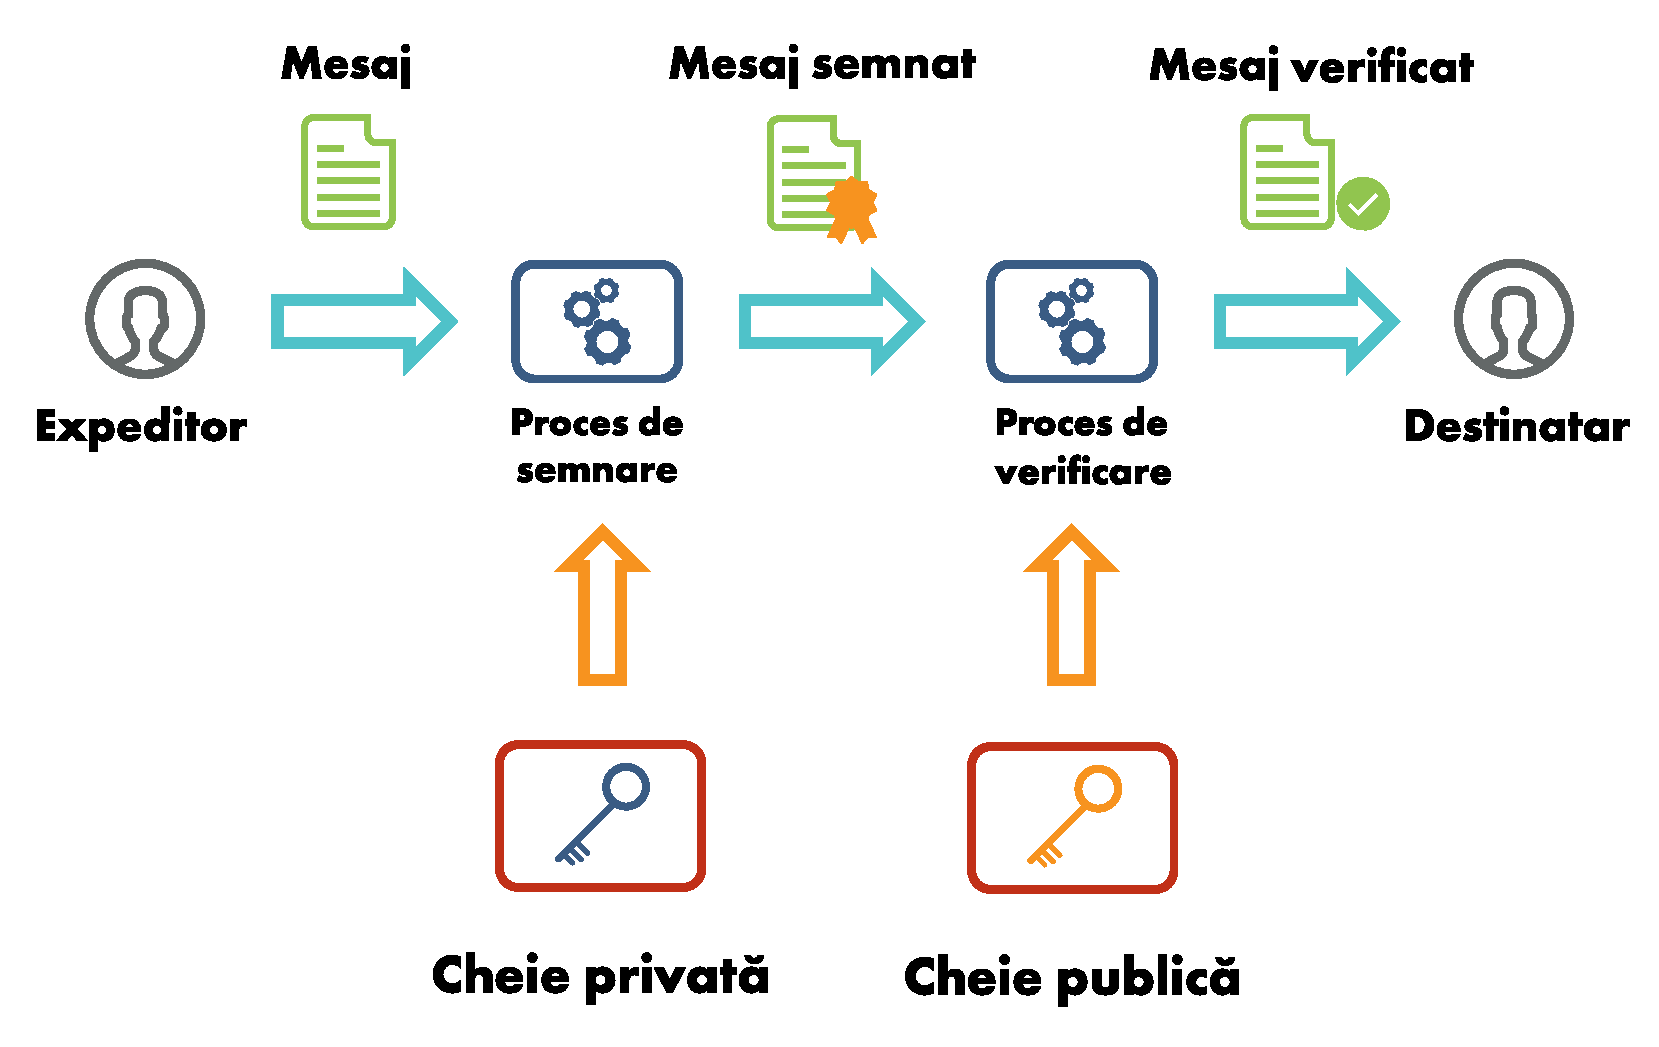
\includegraphics[width=0.7\textwidth]{chapters/12-auth/img/digital-signature.svg.pdf}
  \caption{Digital signing and verification}
  \label{fig:sec:digital-signature}
\end{figure}

Following the signing process with the private key results in a digital signature, a string of bytes resulting from the signing.
The signed document is then exposed publicly, along with the signature.
The public key is already public.
Anyone can then take the document together with the digital signature and verify, using the public key, the authenticity of the document.
This is a way that can be used for electronic mail messages (e-mails) to guarantee that a message is the correct one, having the signature attached.
Or it is a way in which documents can be signed, without the physical presence of signatories or the physical form of a document being necessary.
For signatures in e-mails and for document signatures, in Linux we can use the GPG \abbrev{GPG}{GNU Privacy Guard} (\textit{GNU Privacy Guard}) utility.

In the form presented above, digital signatures only certify the authenticity of the message, that is, it is an authentic signed message.
But they do not certify the identity of the signer.
They can claim to be another person, generate a private key - public key pair and sign messages using the private key while others can verify using the public key.
For this, we need a way to attach a physical identity (name, email) to a public key and to have trust that that attachment is valid;
that is, indeed the identity is that of the claimed person and it is their public key.

The association of an identity with a public key is called a digital identity certificate or public key certificate or simply \textbf{digital certificate}.
For the association to be valid, the certificate must be signed by an entity in which we have trust, as we specified above in \labelindexref{Section}{sec:sec:transfer:identity}.
Depending on the nature of this entity, we have a centralized form, called Public Key Infrastructure (\textit{Public Key Infrastructure}) and a decentralized form, called web of trust (\textit{web of trust}).

\subsubsection{Public Key Infrastructure}
\label{sec:sec:transfer:sign:pki}

In the case of the centralized form, there is a separate entity in which we have trust called \textbf{Certification Authority} (\textit{Certificate Authority} - CA\abbrev{CA}{Certificate Authoriry}).
Similar to an authorized ministry that certifies a person's identity on a document, the certification authority is the one that signs a certificate that associates the identity with a public key.
We thus have a Public Key Infrastructure (\textit{Public Key Infrastructure} - PKI\abbrev{PKI}{Public Key Infrastructure}).
The steps followed for verifying a signed document in PKI are presented in \labelindexref{Figure}{fig:sec:pki}:

\begin{enumerate}
  \item The client connects to the server to access the desired resource.
  \item The server presents its certificate to the client.
    Now the client has access to the server's certificate (and to the certification authority's certificate - CA).
  \item The client extracts the certification authority's public key from its certificate.
  \item The client verifies, using the certification authority's public key, the server's certificate.
    If the verification succeeded, now the client has trust in the server's identity and can communicate securely with it.
  \item (optional) The server requests the client's certificate to verify its identity.
    Mirroring step 1.
  \item (optional) The client presents its certificate to the server.
    Now the server has access to the client's certificate (and to the certification authority's certificate - CA).
    Mirroring step 2.
  \item (optional) The server extracts the certification authority's public key from its certificate.
    Mirroring step 3.
  \item (optional) The server verifies, using the certification authority's public key, the client's certificate.
    If the verification succeeded, now the server has trust in the client's identity and can communicate securely with it.
    Mirroring step 4.
    At this moment both entities have verified identities.
  \item The client (or server) presents the encryption key (generally, symmetric) used for ensuring the confidentiality of the current session.
  \item Now the secure communication channel is established and the client can access the desired resource.
\end{enumerate}

Steps 5-8 above are optional steps for verifying the client's identity by the server.
Usually, only the client is interested in the server's identity.
The client's identity is either not relevant to the server (for public resources, such as searching using Google), or uses specialized authentication forms for demonstrating identity (for private/personal resources, such as accessing the Facebook account).

\begin{figure}[htbp]
  \centering
  \begin{subfigure}[b]{0.48\textwidth}
    \centering
    \def\svgwidth{\columnwidth}
    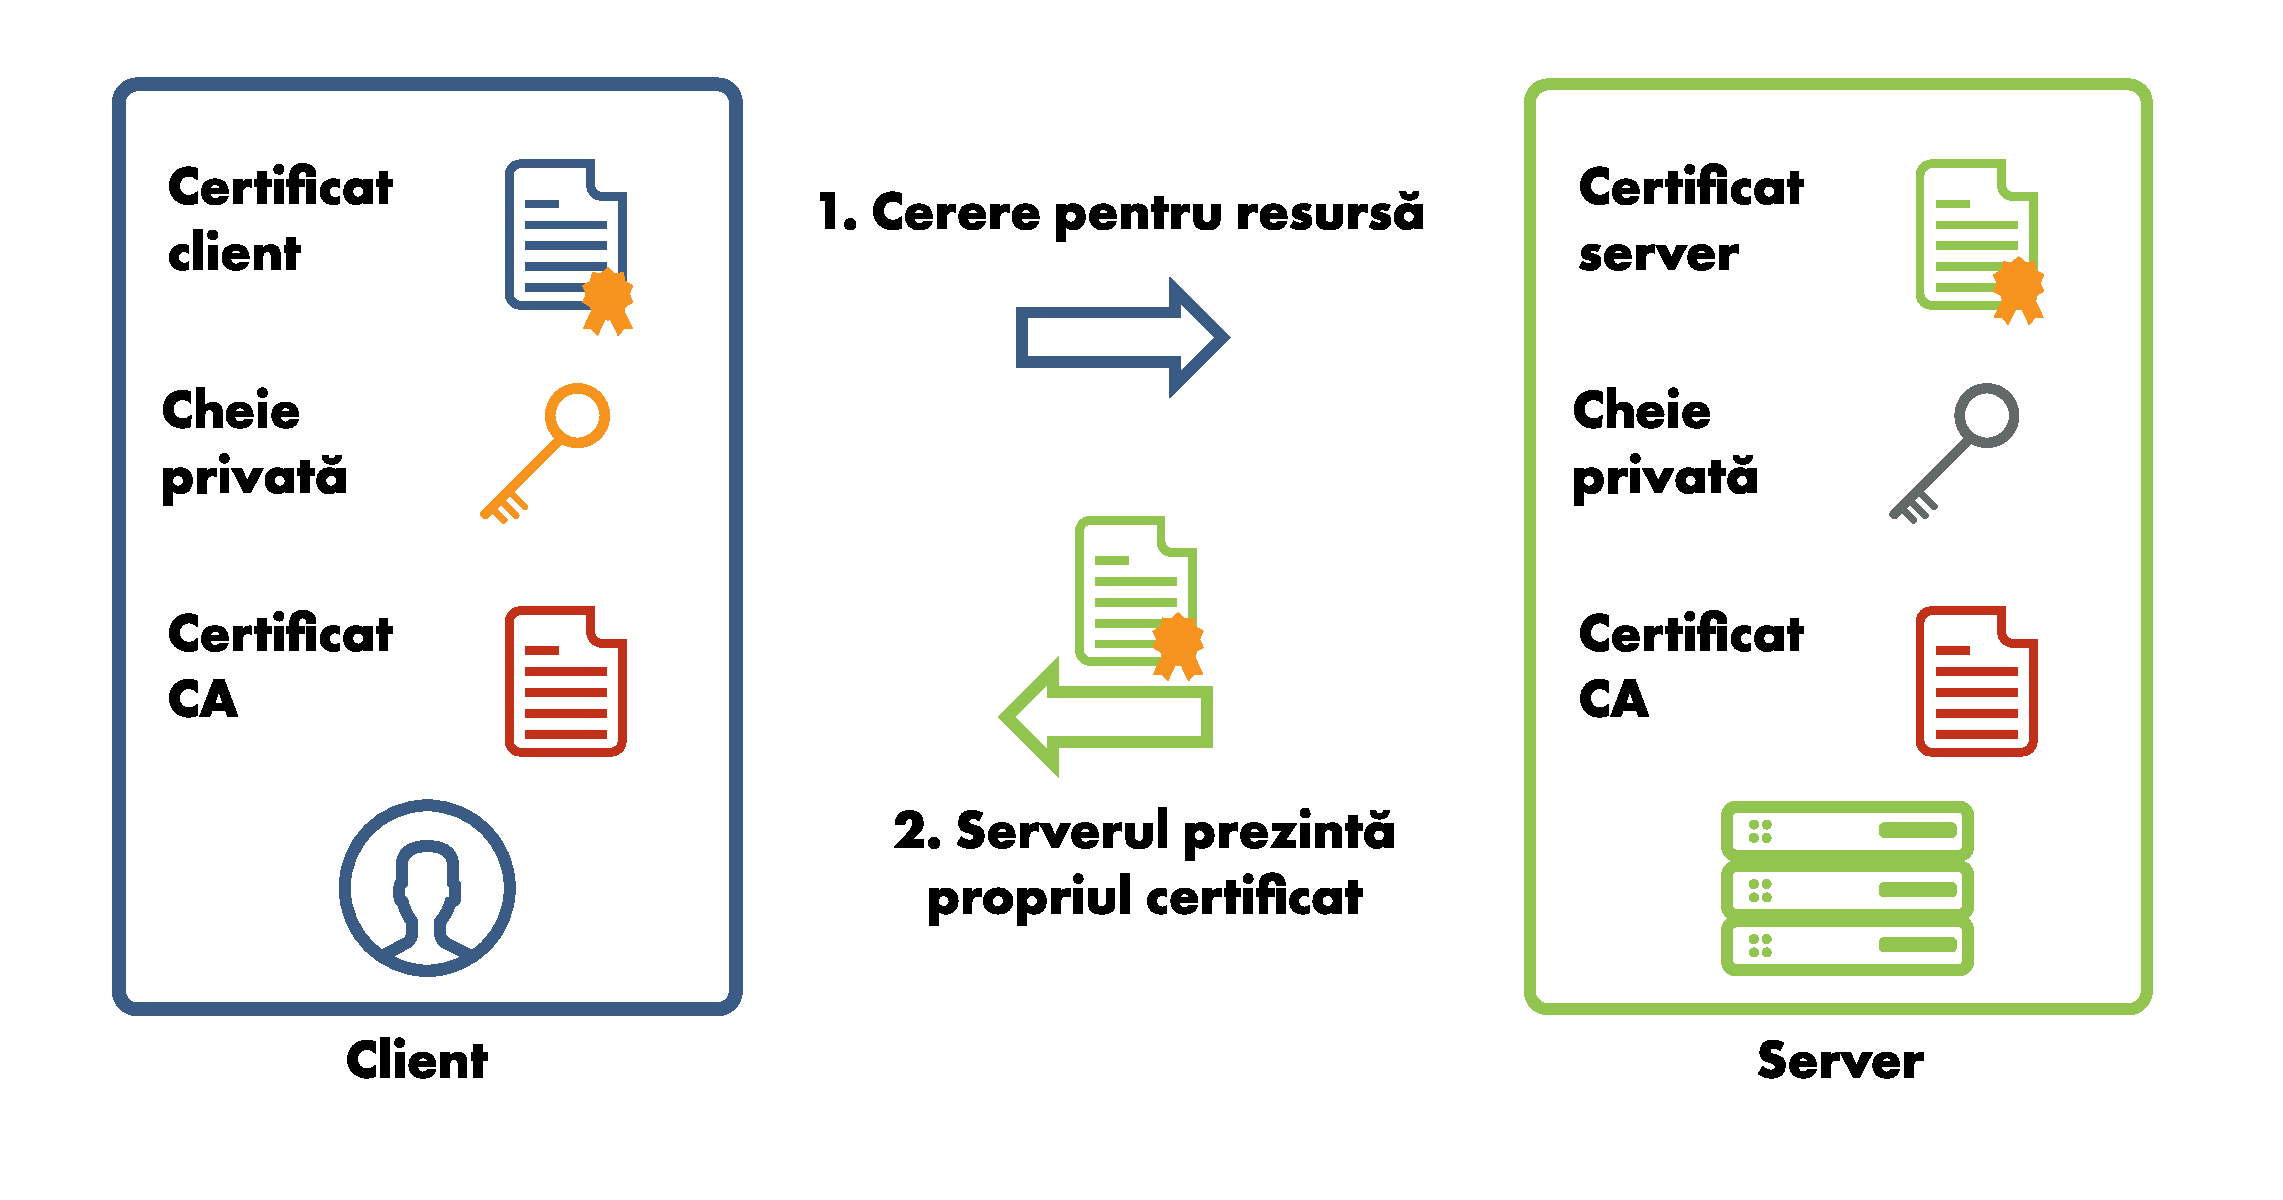
\includegraphics{chapters/12-auth/img/certificate-1-2.svg.pdf}
  \end{subfigure}
  \begin{subfigure}[b]{0.48\textwidth}
    \centering
    \def\svgwidth{\columnwidth}
    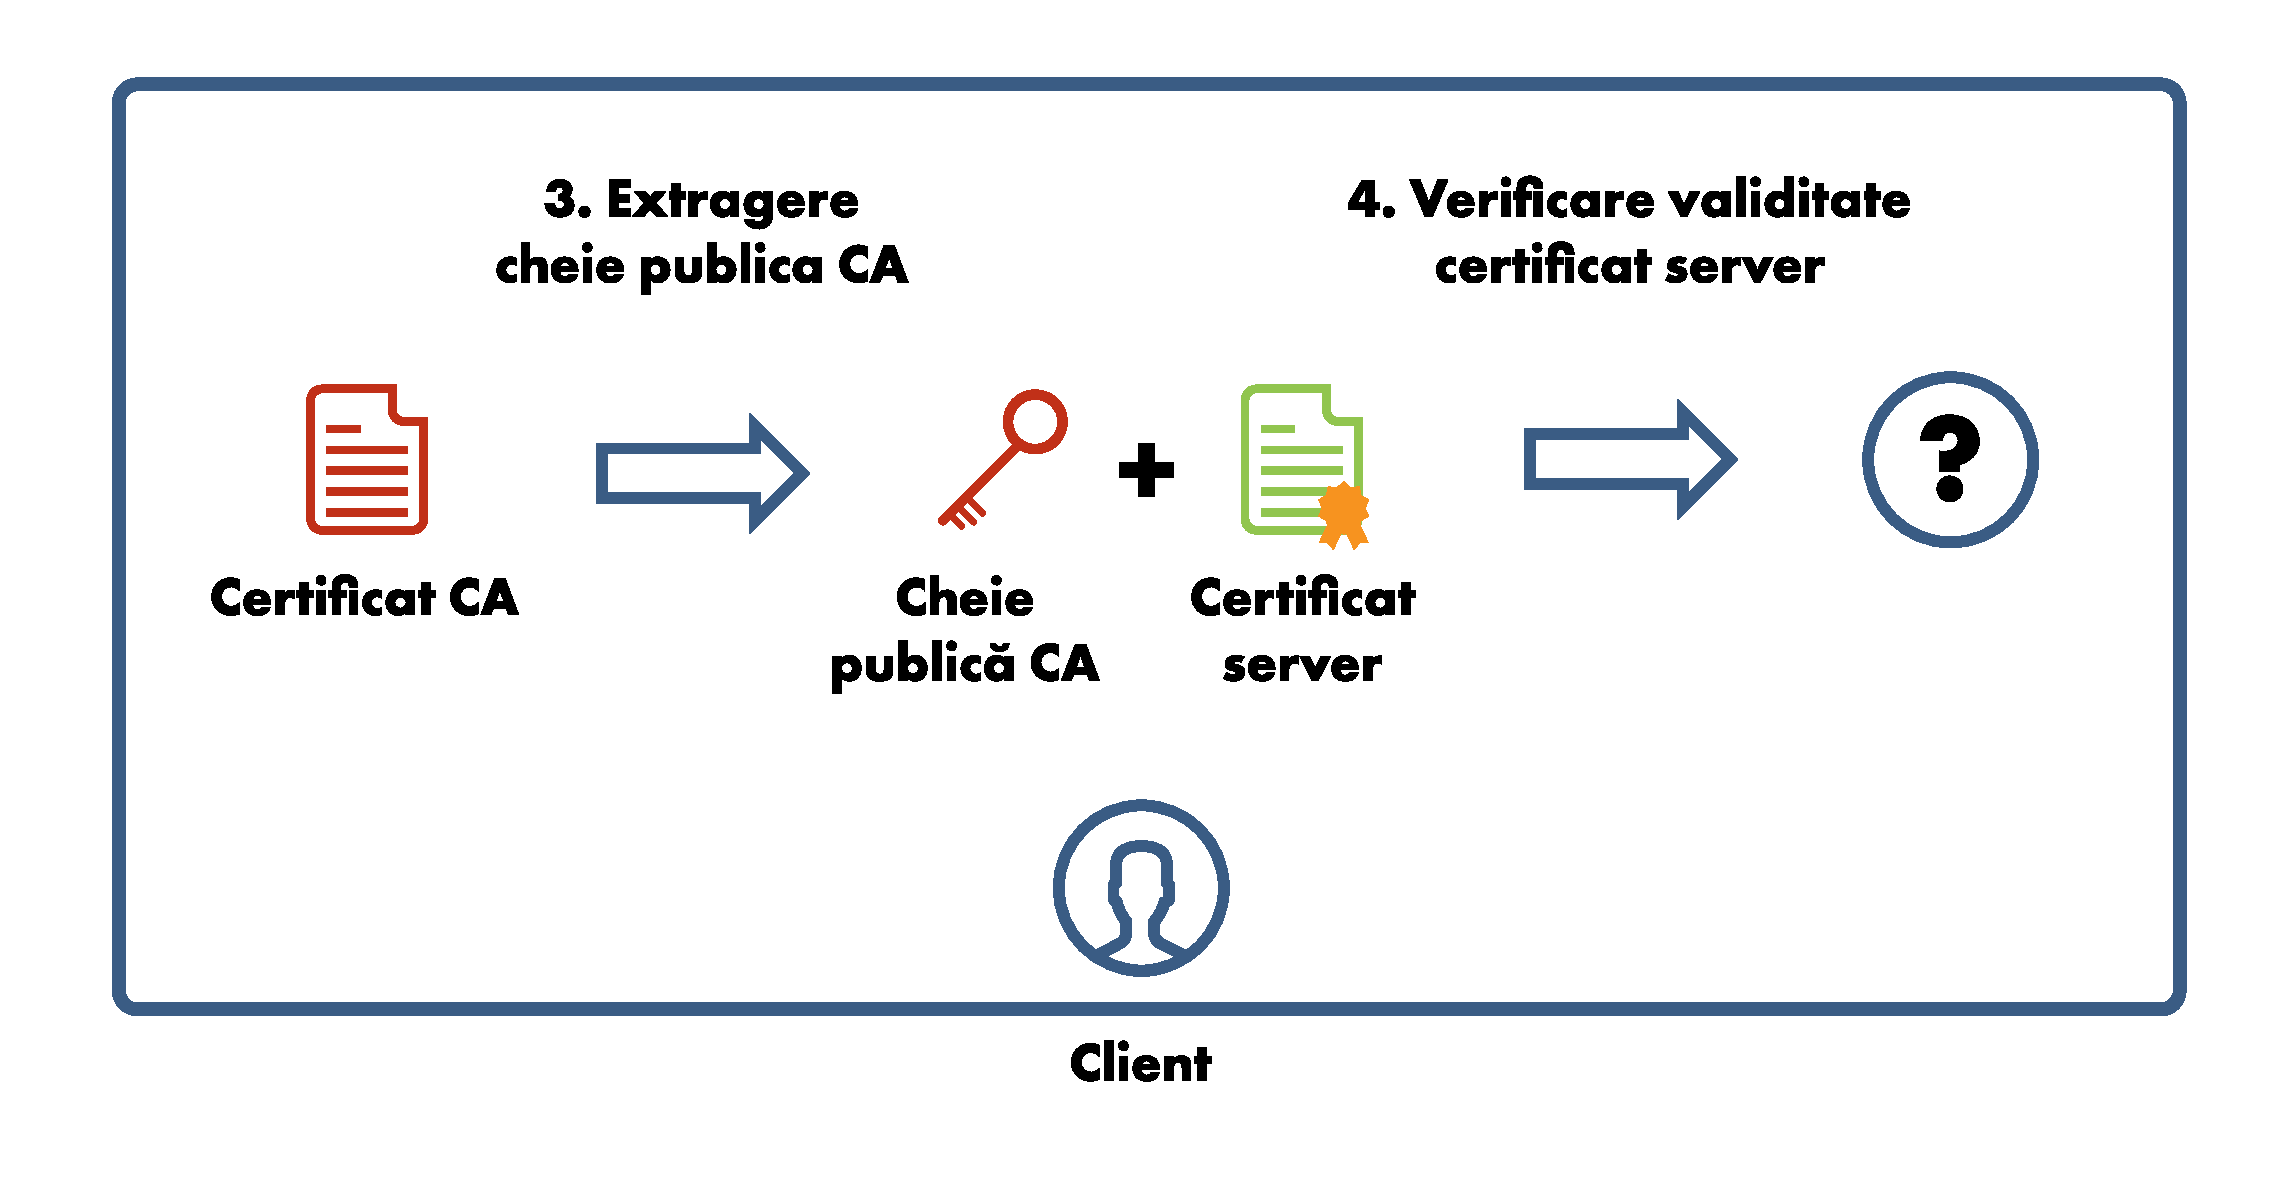
\includegraphics{chapters/12-auth/img/certificate-3-4.svg.pdf}
  \end{subfigure}
  \begin{subfigure}[b]{0.48\textwidth}
    \centering
    \def\svgwidth{\columnwidth}
    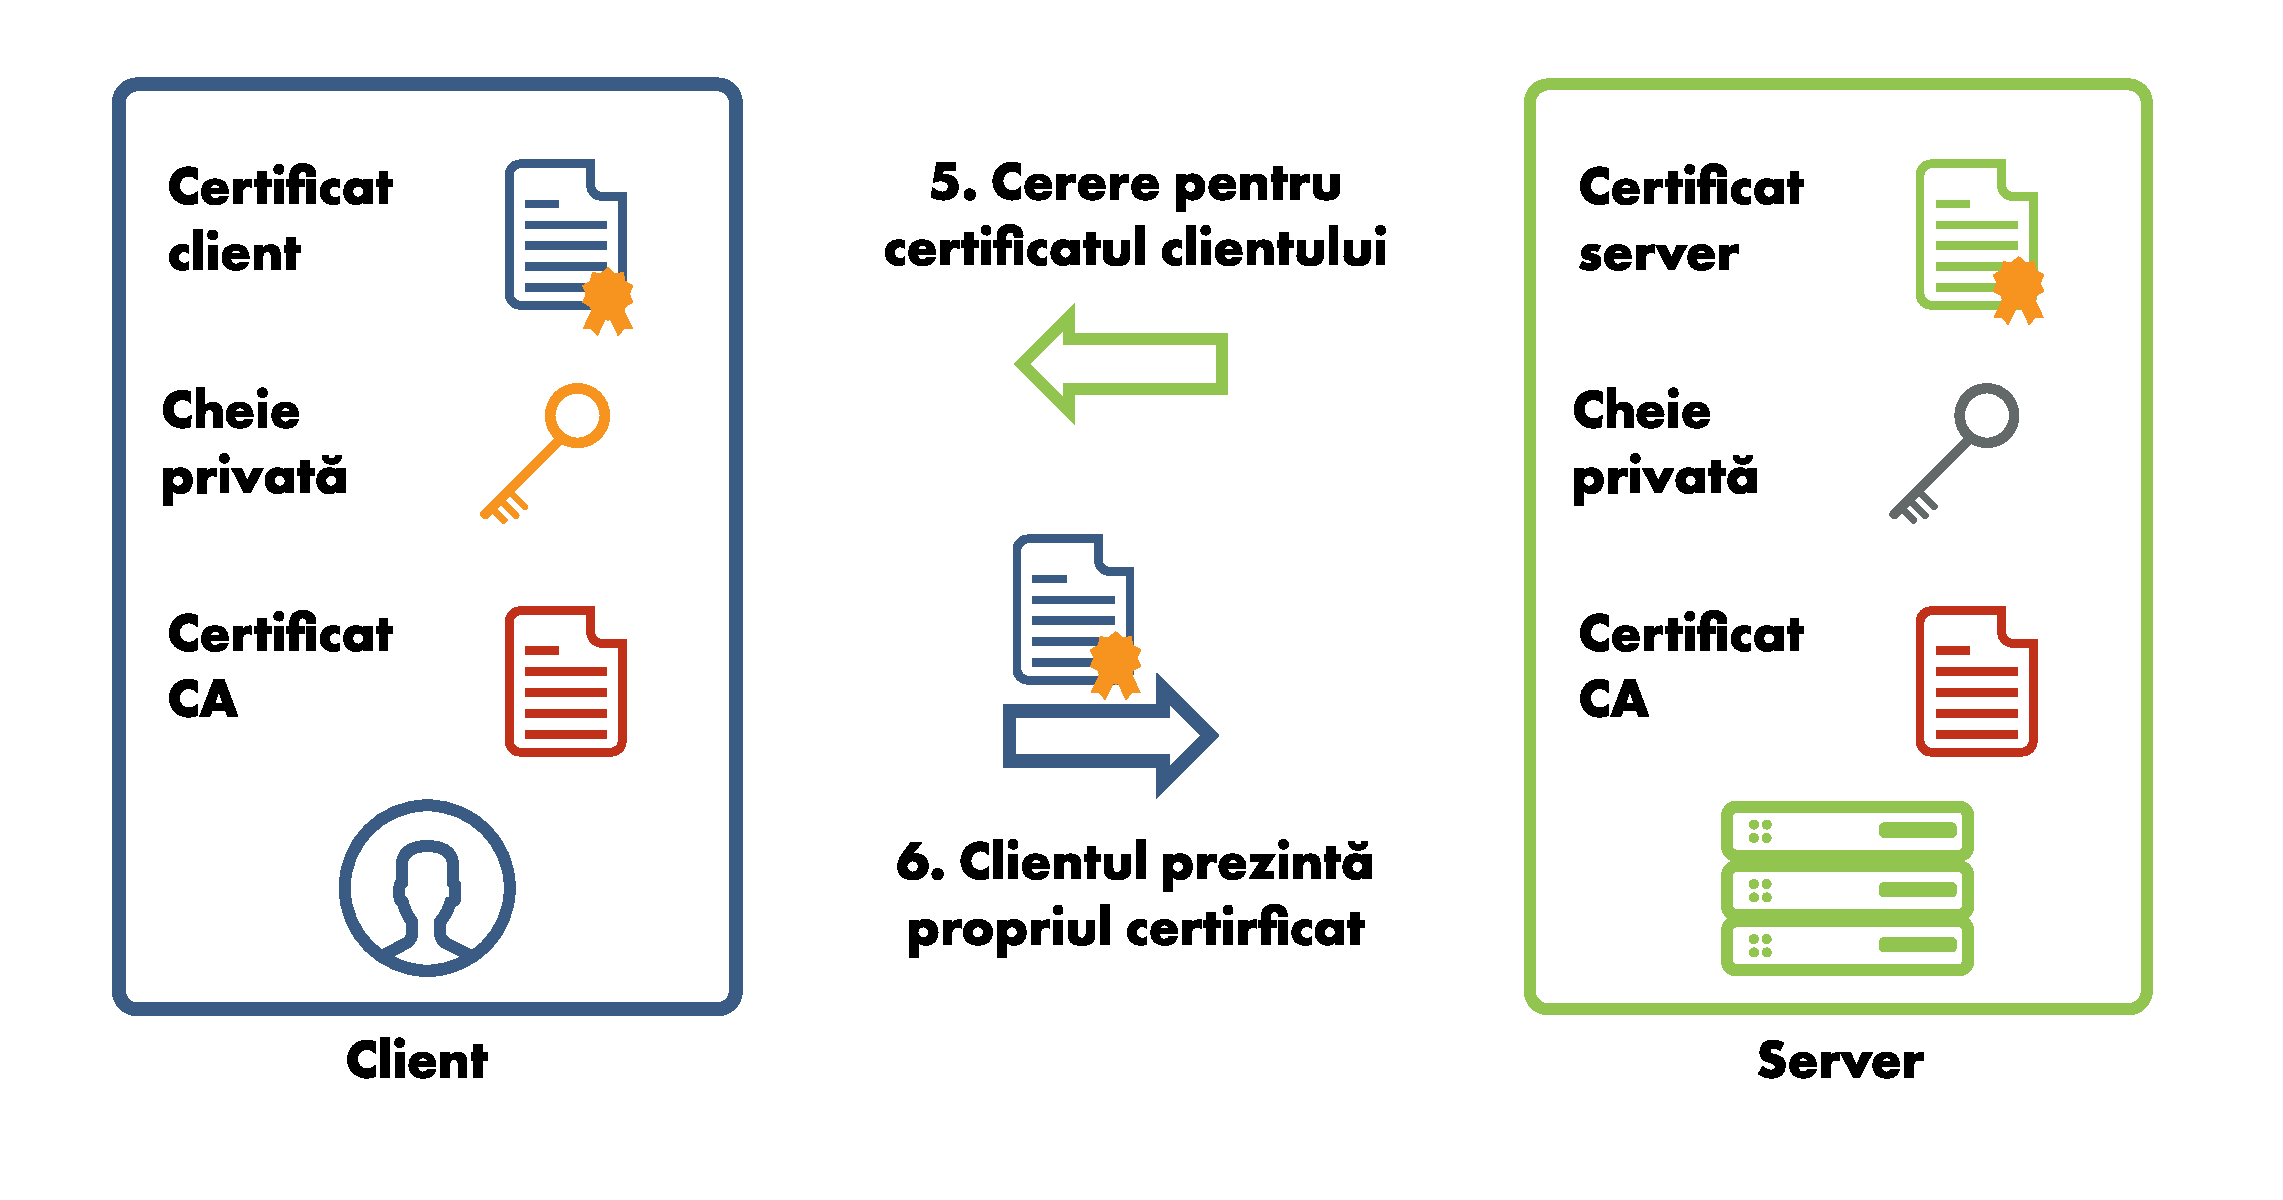
\includegraphics{chapters/12-auth/img/certificate-5-6.svg.pdf}
  \end{subfigure}
  \begin{subfigure}[b]{0.48\textwidth}
    \centering
    \def\svgwidth{\columnwidth}
    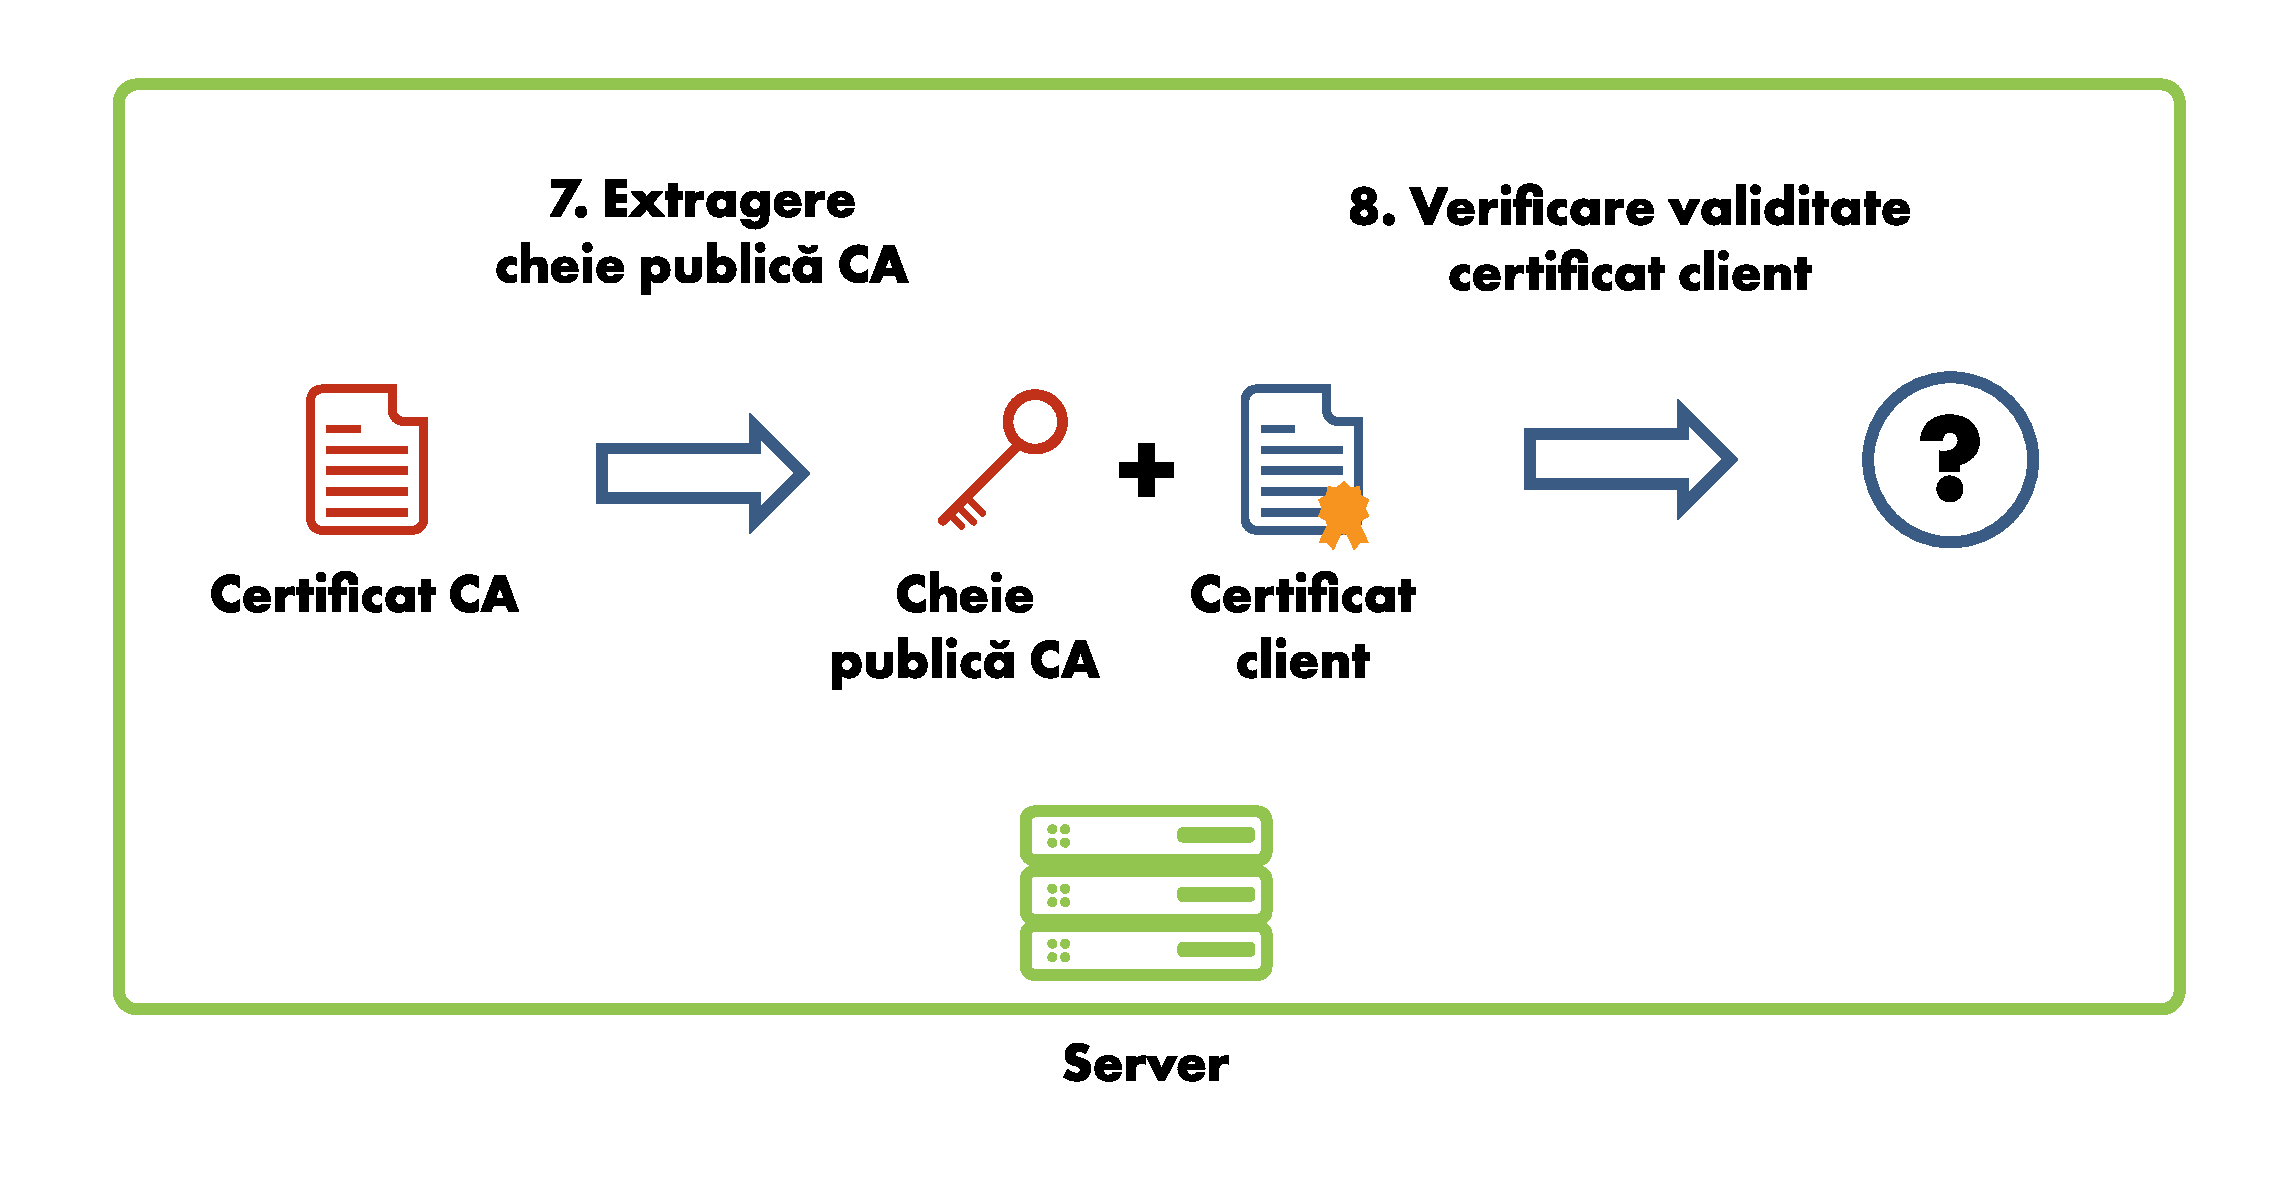
\includegraphics{chapters/12-auth/img/certificate-7-8.svg.pdf}
  \end{subfigure}
  \begin{subfigure}[b]{0.48\textwidth}
    \centering
    \def\svgwidth{\columnwidth}
    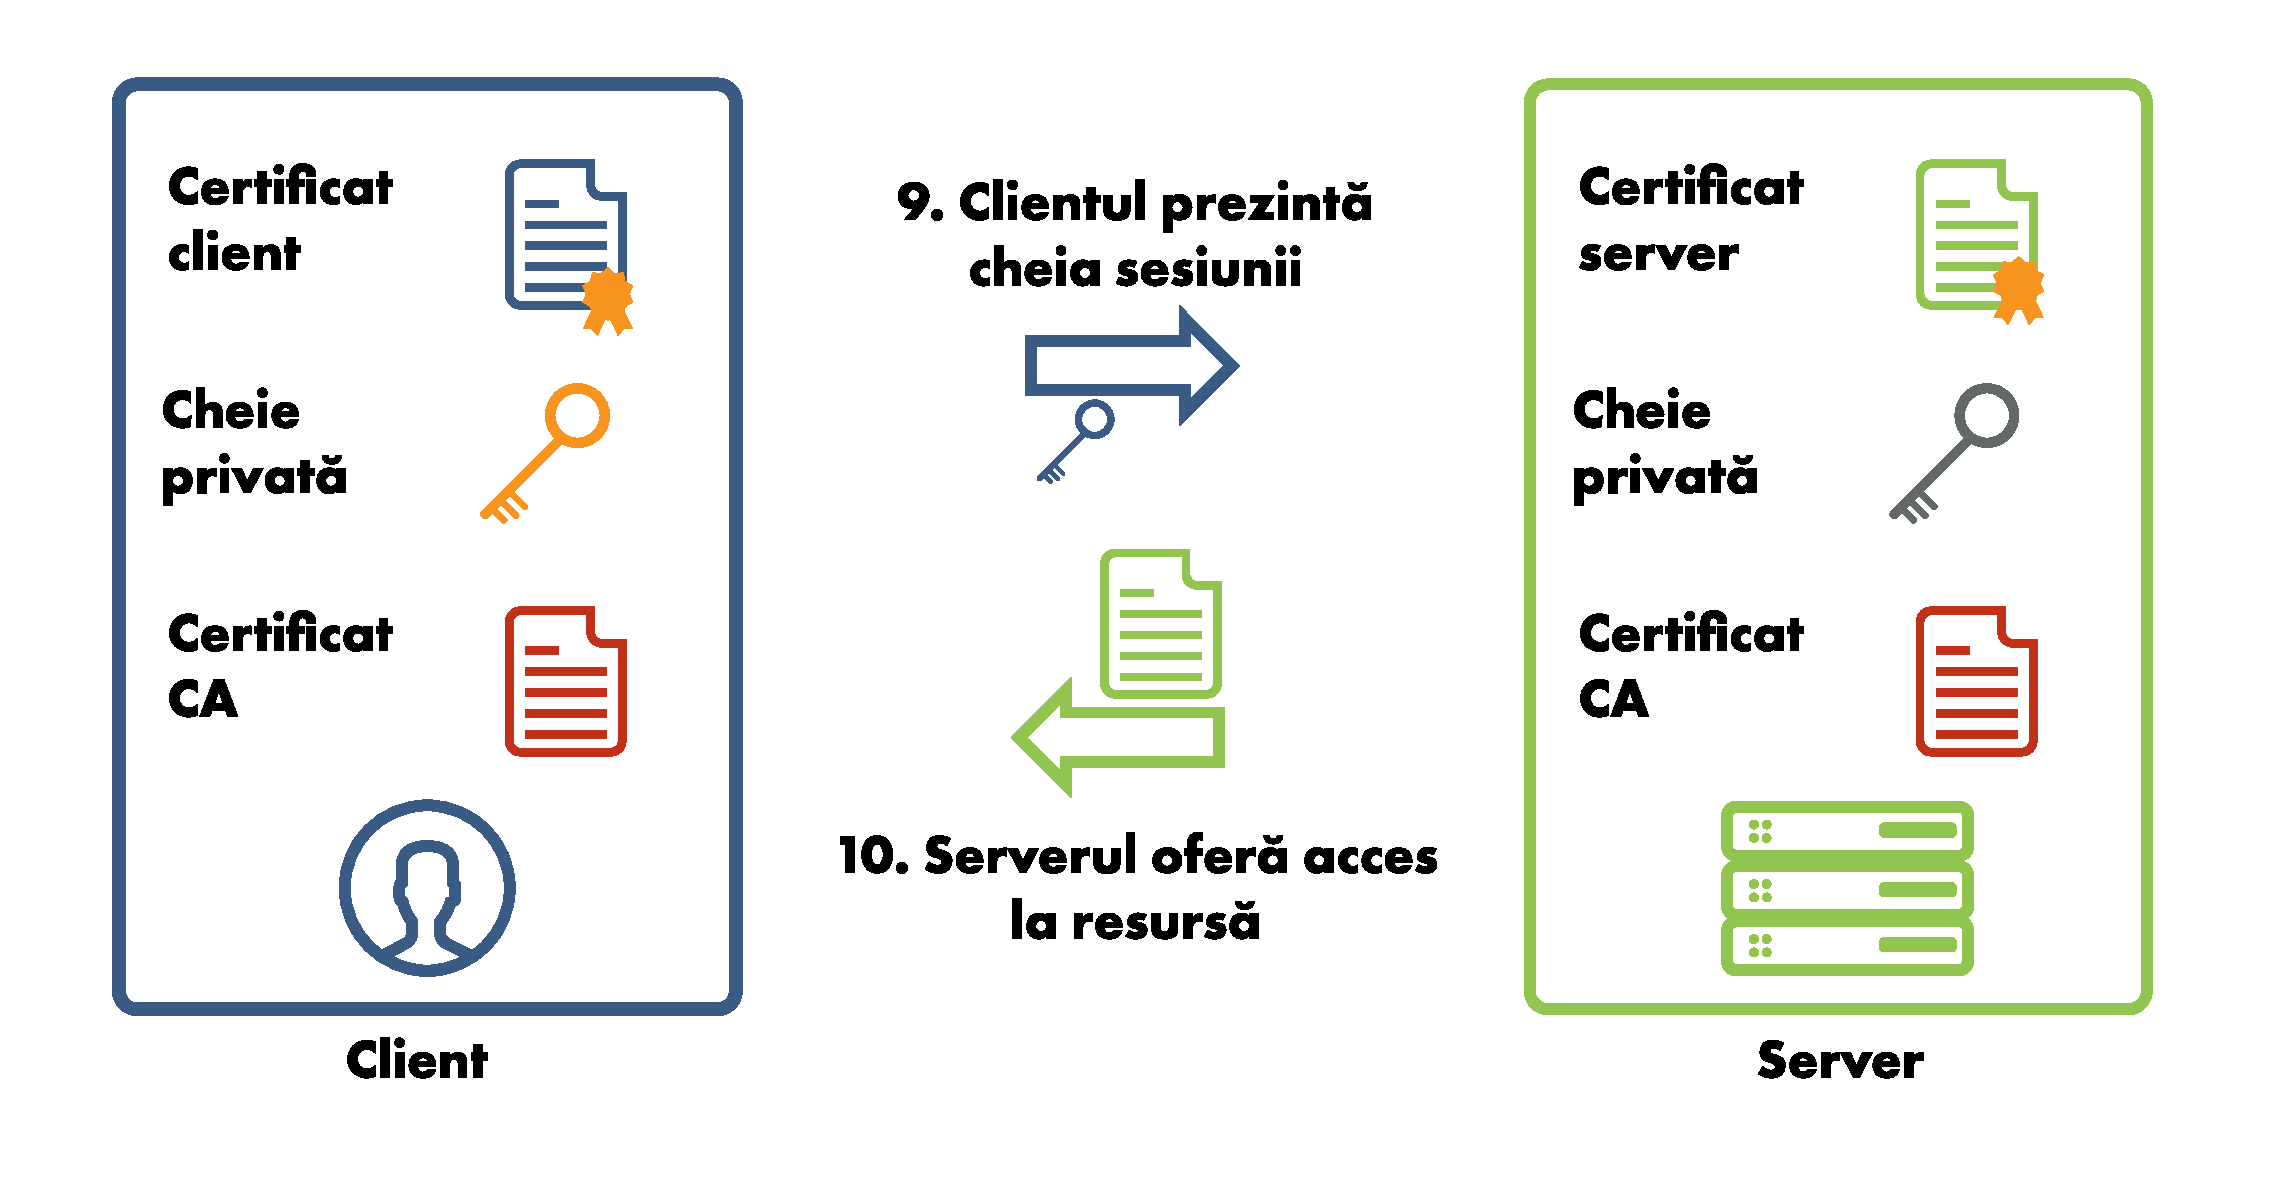
\includegraphics{chapters/12-auth/img/certificate-9-10.svg.pdf}
  \end{subfigure}
  \caption{Identity verification in PKI}
  \label{fig:sec:pki}
\end{figure}

When we want to verify a document, we will obtain the signer's digital certificate, we will verify the digital certificate using the public key (in which we have trust) of the certification authority.
If the digital certificate is valid, we will extract the public key from it and then verify the signature.
Having the digital certificate verified by the certification authority, we have trust that the identity is the one in the certificate.

In the PKI scheme, we must have trust in the certification authority.
We will have access to its public key and we will have trust that that public key is indeed that of the certification authority.
The public key is used for verifying certificates.
This public key of the certification authority is itself distributed in the form of a certificate.
This certificate can be signed by another higher-level CA entity.
At some point, there will be a certification authority that will no longer be signed by another, it is said that we have reached the root of the PKI scheme.
This certification authority will have a root certificate (\textit{root certificate}) which is signed by itself (\textit{self signed}).
That is, its own private key is used to sign the certificate that contains its own public key and identity.

The PKI scheme is used on the Internet to guarantee the identity of the sites we visit (google.com, facebook.com, amazon.com).
Each site has a digital certificate signed by a certification authority in which we have trust.
When we install a browser, it already has the certificates of various certification authorities and can verify the authenticity of certificates provided by different sites and, therefore, their identity.

Also, the PKI scheme is used for electronic signatures of documents.
The strongest form is called \textbf{qualified electronic signature} (\textit{qualified electronic signature}).
This form is considered in the legislation of many countries as being equivalent to the written signature (holographic).
In general, obtaining a qualified electronic signature requires obtaining an electronic signature device (token).
This token stores the private key used for signing.
The private key cannot be used in the absence of this token and, therefore, the electronic signature cannot be realized.
In general, the token is obtained at a cost from a company authorized as an electronic signature provider.
Most often, the token connects to the USB port of a laptop/desktop for signing documents from that system.

\subsubsection{Web of Trust}
\label{sec:sec:transfer:sign:wot}

The PKI scheme is a centralized scheme.
It has the advantage of organization and the existence of a chain of trust and responsibility.
However, if a certification authority is compromised, then all certificates signed by it are compromised.
That is why certificates have a limited lifetime (usually 1-2 years) after which they must be regenerated.

The alternative to the centralized PKI scheme is the decentralized \textbf{web of trust} scheme.
In this scheme, each user knows certain users directly (knows them physically), can guarantee them and signs each one's certificates.
Then this user, based on direct connections, can accept certificates signed by these direct connections.
They do not know the end users directly but have trust in the signatures of their direct connections.
The functioning of web of trust is described schematically in \labelindexref{Figure}{fig:sec:web-of-trust}.

\begin{figure}[htbp]
  \centering
  \def\svgwidth{\columnwidth}
  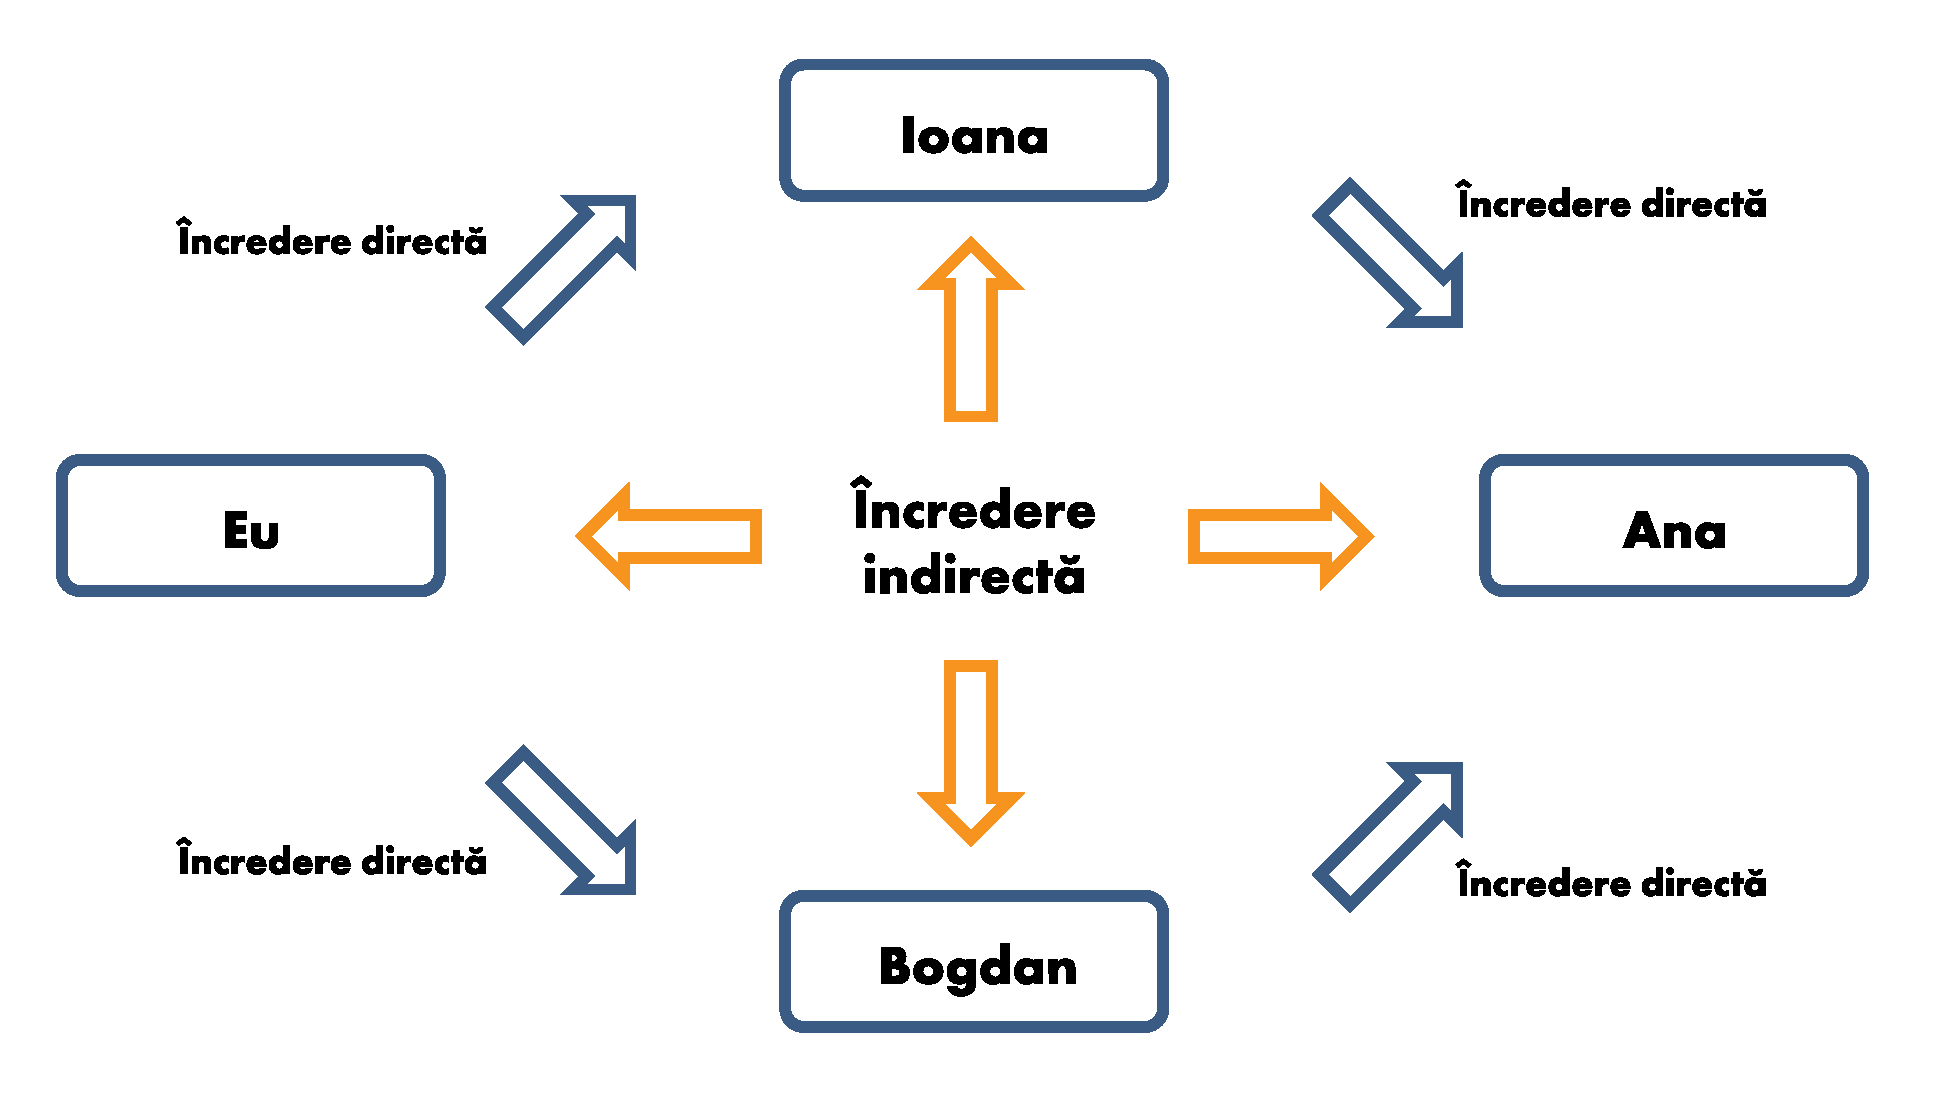
\includegraphics[width=0.7\textwidth]{chapters/12-auth/img/web-of-trust.svg.pdf}
  \caption{Web of Trust Functioning}
  \label{fig:sec:web-of-trust}
\end{figure}

The advantage of the web of trust scheme over PKI is flexibility.
Not having a central authority, we do not have the rigidity of the PKI scheme.
A disadvantage of it is the difficulty of verifying proper functioning.
In the absence of a rigorous structure, verifying proper functioning is cumbersome.
For this reason, real large-scale implementations of web of trust are more limited.
A common implementation is signing e-mails using implementations from the PGP \abbrev{PGP}{Pretty Good Privacy} (\textit{Pretty Good Privacy}) family such as the GPG utility presented above.

\subsection{Transport Layer Security (TLS)}
\label{sec:sec:transfer:tls}

For ensuring the properties mentioned at the beginning of the chapter (confidentiality, authenticity/identity, and integrity), modern network protocols incorporate \textit{Transport Layer Security} (TLS\abbrev{TLS}{Transport Layer Security}), also known in its old name as \textit{Secure Sockets Layer} - SSL\abbrev{SSL}{Secure Sockets Layer}.
TLS is a cryptographic security framework used for securing network traffic.
For example, the HTTP protocol (\textit{Hypertext Transfer Protocol}) does not have security features, however, if we attach TLS to it, the protocol becomes secure in its HTTPS \abbrev{HTTPS}{Hypertext Transfer Protocol secure} (\textit{Hypertext Transfer Protocol Secure}) variant.

TLS incorporates most of the concepts we described in this section: it uses digital certificates to certify the identity of the conversation partner, uses key exchange protocols such as Diffie-Hellman, uses symmetric key protocols such as AES, uses hashing algorithms such as SHA-2.
Within a TLS session, the client and server agree on which algorithms to use based on each one's capabilities.

The current version of TLS is 1.3 (from August 2018) and is considered secure.
Previous versions present algorithm vulnerabilities.
In general, a newer TLS specification means that certain algorithms are no longer allowed, or encryption keys are longer, precisely to prevent their exploitation.
Usually, it is recommended that a server refuse connections that request weaker algorithms that can then be exploited.
This type of attack is called \textit{connection downgrade attack} and is used to impose a weaker algorithm that is known to have vulnerabilities.

If we want to verify the TLS security level for a web server we have configured (or another), we can use test applications such as SSL Server Test\footnote{\url{https://www.ssllabs.com/ssltest/}}, as presented in \labelindexref{Figure}{fig:sec:ssllabs}.
In such a test, we are reported the weak points of a server, such as the fact that it accepts TLS 1.1 and TLS 1.2 connections which can have problems for certain algorithms.

\begin{figure}[!htbp]
  \centering
  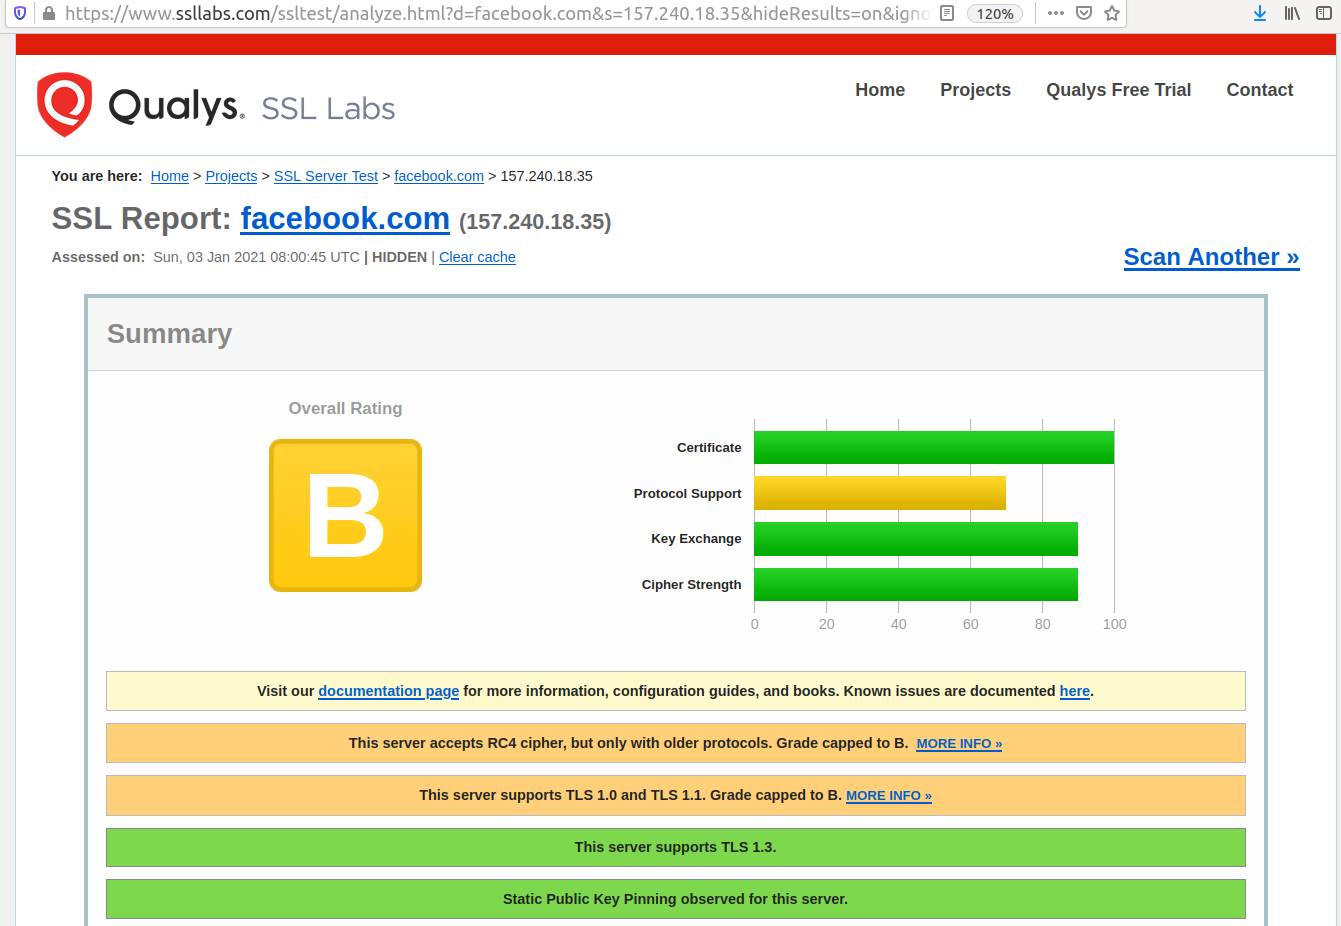
\includegraphics[width=0.8\textwidth]{chapters/12-auth/img/ssllabs.png}
  \caption{Verifying the security level for a domain}
  \label{fig:sec:ssllabs}
\end{figure}

Similar to encryption functionalities, TLS is usually implemented in the form of cryptographic libraries.
Insecure protocols use TLS to obtain their secure form: these are HTTP/HTTPS (for web access), IMAP/IMAPS (for mailbox access), LDAP/LDAPS (for querying information directories).

The OpenSSL library, which we mentioned in \labelindexref{Section}{sec:sec:data:confidentiality}, implements TLS and is used by many network applications to communicate securely.
The command-line utility \cmd{openssl} allows, for test scenarios, building or verifying a secure connection.
For example, the command in \labelindexref{Listing}{lst:sec:openssl-check} obtains information about the digital certificate used by the \texttt{google.com} server.

\begin{screen}[caption={Obtaining information about a domain's certificate},label={lst:sec:openssl-check}]
student@uso:~$ openssl s_client -connect google.com:443
CONNECTED(00000005)
depth=2 OU = GlobalSign Root CA - R2, O = GlobalSign, CN = GlobalSign
verify return:1
depth=1 C = US, O = Google Trust Services, CN = GTS CA 1O1
verify return:1
depth=0 C = US, ST = California, L = Mountain View, O = Google LLC, CN = *.google.com
verify return:1
---
Certificate chain
 0 s:C = US, ST = California, L = Mountain View, O = Google LLC, CN = *.google.com
   i:C = US, O = Google Trust Services, CN = GTS CA 1O1
 1 s:C = US, O = Google Trust Services, CN = GTS CA 1O1
   i:OU = GlobalSign Root CA - R2, O = GlobalSign, CN = GlobalSign
---
Server certificate
-----BEGIN CERTIFICATE-----
[...]
\end{screen}

\subsection{Secure Shell}
\label{sec:sec:transfer:ssh}

Transport Layer Security (TLS) allows adding security properties for protocols in a library implementation.
An alternative to TLS for creating a secure communication channel is the SSH (\textit{Secure Shell}) protocol.
The SSH protocol, like TLS, offers confidentiality, integrity, and authenticity.
The SSH protocol is generally used for opening a secure remote shell connection on an encrypted channel.
It thus allows remote administration of a system.
It is, therefore, the main utility used in the Linux/Unix world for system administration and is present on most server-type systems.

Despite its name, the SSH protocol is not used only for opening a secure remote shell session;
the SSH protocol creates a secure communication channel through which actions such as opening a remote shell session, file transfer, or tunneling a protocol can be performed, also described in \labelindexref{Figure}{fig:sec:ssh-channel}.
Tunneling an insecure protocol (of \textit{plaintext} type) means that messages specific to this protocol are passed through the secure connection channel established by SSH.
In this way, SSH offers functionality similar to TLS, of securing a protocol.
However, in TLS, the protocol in its secure form is already implemented, while in the case of SSH, it is necessary to create the secure communication channel through which the insecure protocol is then tunneled.
Since it is simpler to use, we prefer using the secure protocol using TLS;
SSH remains useful however in situations where we do not have the secure form of the protocol through TLS, such as tunneling the X protocol for the graphical environment in Linux, as we presented in \labelindexref{Section}{sec:ui:window-system}.

\begin{figure}[htbp]
  \centering
  \def\svgwidth{\columnwidth}
  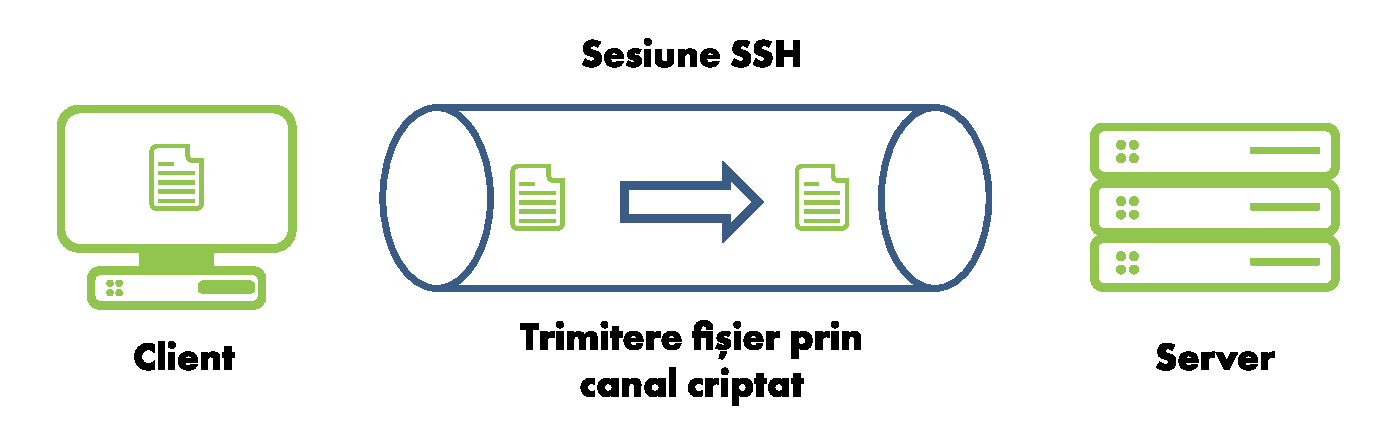
\includegraphics[width=0.7\textwidth]{chapters/12-auth/img/ssh-channel.svg.pdf}
  \caption{Secure communication channel with SSH}
  \label{fig:sec:ssh-channel}
\end{figure}

\begin{figure}[htbp]
  \centering
  \def\svgwidth{\columnwidth}
  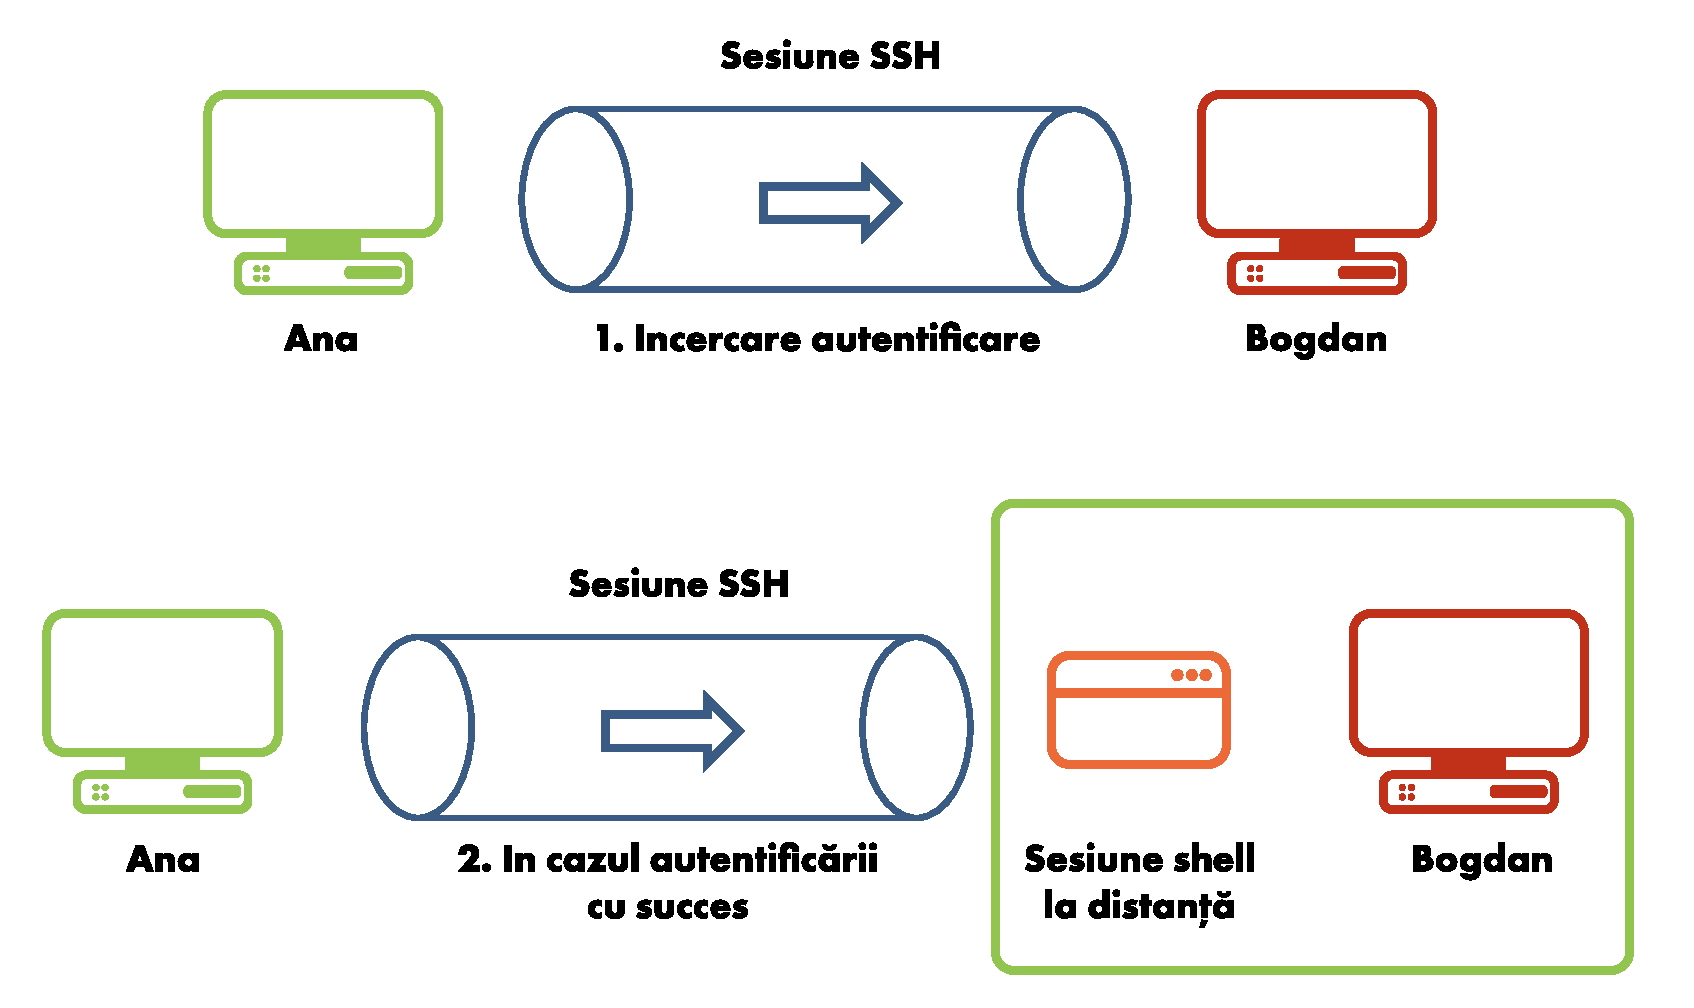
\includegraphics[width=0.7\textwidth]{chapters/12-auth/img/ssh-session.svg.pdf}
  \caption{SSH Connection}
  \label{fig:sec:ssh-session}
\end{figure}

To function, the SSH protocol needs a user account at the source and destination.
Practically, we establish a secure communication channel between two user accounts, usually for opening a remote shell session, as in \labelindexref{Figure}{fig:sec:ssh-session}.
Channel creation is performed only after authentication on the destination account.
Authentication can be performed with a password or using a public key, as we describe further.
Once authentication is completed, we have a communication channel through which we can tunnel commands (in the case of the shell), files (in the case of file transfer), or protocols.

For establishing an SSH connection, an SSH server must be running at the destination, also called SSH daemon.
The SSH server usually runs on port 22, its presence can be verified using the \cmd{netstat} utility as in \labelindexref{Listing}{lst:sec:ssh-netstat}.

\begin{screen}[caption={SSH Server},label={lst:sec:ssh-netstat}]
student@uso:~$ netstat -tln | grep 22
tcp        0      0 0.0.0.0:22              0.0.0.0:*               LISTEN
tcp6       0      0 :::22                   :::*                    LISTEN
\end{screen}

If the SSH server is not present, it is possible that it is stopped or not installed.
For installing and starting/restarting the SSH server we use the commands from \labelindexref{Listing}{lst:sec:ssh-server}.
The installation commands are respectively for Debian/Ubuntu systems and for RedHat/Fedora systems.

\begin{screen}[caption={Install and start SSH server},label={lst:sec:ssh-server}]
# Install SSH server on Debian / Ubuntu.
student@uso:~$ sudo apt install openssh-server

# Install SSH server on RedHat / Fedora.
student@uso:~$ sudo dnf install openssh-server

# Restart SSH server.
student@uso:~$ sudo systemctl restart ssh
\end{screen}

For opening a remote shell session we use the \cmd{ssh} command followed by the destination: the username and the destination station address;
the destination station address can be IP address or DNS name.
In \labelindexref{Listing}{lst:sec:ssh-shell} we have examples of remote connections.
The remote user's password is requested and, in case of a successful connection, a shell is obtained that runs remotely with the remote user's permissions.
For closing the connection, we close the shell process using the \cmd{exit} or \cmd{logout} commands or the \texttt{Ctrl+d} key combination.

\begin{screen}[caption={Remote shell access using SSH},label={lst:sec:ssh-shell}]
student@uso:~$ ssh malus@vmx.cs.pub.ro
malus@vmx.cs.pub.ro's password:
[...]
malus@vmx:~$ ls
extra  from-upb-to-ncsu  iOracle.git  ios-privacy-leaks  lib  prolog-data  prolog-query-work  pwn3  scripts
malus@vmx:~$ exit
logout
Connection to vmx.cs.pub.ro closed.
student@uso:~$
\end{screen}

The remote connection command can be followed by another command, in which case an interactive shell session will not be opened, but that command will be run and then the connection will be closed.
In \labelindexref{Listing}{lst:sec:ssh-commands} we run remotely the \cmd{ls} command or a more complex command to quickly get information from that system without needing to open an interactive shell session.

\begin{screen}[caption={Running remote commands through SSH},label={lst:sec:ssh-commands}]
student@uso:~$ ssh malus@vmx.cs.pub.ro ls
malus@vmx.cs.pub.ro's password:
extra
from-upb-to-ncsu
iOracle.git
ios-privacy-leaks
lib
prolog-data
prolog-query-work
pwn3
scripts
student@uso:~$ ssh malus@vmx.cs.pub.ro hostname
malus@vmx.cs.pub.ro's password:
vmx.cs.pub.ro
\end{screen}

When we make a connection to a remote system for the first time, we will receive a warning message that the identity of that system is not known and we are asked if we want to continue.
If we answer affirmatively and continue, the public key (identity) of that system will be added to a specific configuration file (\file{$\sim$/.ssh/known\_hosts}) and we will not receive the question later.
In \labelindexref{Listing}{lst:sec:ssh-host-check} the file \file{$\sim$/.ssh/known\_hosts} does not exist, then at the first connection we receive the question and answer affirmatively;
the file \file{$\sim$/.ssh/known\_hosts} now has the corresponding entry for the remote system (the public key), and at the next connection we no longer receive the question, since we know the server's identity.

\begin{screen}[caption={Verifying server identity through SSH},label={lst:sec:ssh-host-check}]
student@uso:~$ ssh malus@vmx.cs.pub.ro
The authenticity of host 'vmx.cs.pub.ro (141.85.227.139)' can't be established.
RSA key fingerprint is SHA256:CrRMD7nrflw7/KEZ4z7lksvEd8tXxkjuVXoBqsG5Vdc.
Are you sure you want to continue connecting (yes/no)? yes
Warning: Permanently added 'vmx.cs.pub.ro,141.85.227.139' (RSA) to the list of known hosts.
malus@vmx.cs.pub.ro's password:
[...]
malus@vmx:~$ logout
Connection to vmx.cs.pub.ro closed.

student@uso:~$ ssh malus@vmx.cs.pub.ro
malus@vmx.cs.pub.ro's password:
[...]
malus@vmx:~$
\end{screen}

\subsubsection{File Transfer through SSH}
\label{sec:sec:transfer:ssh:transfer}

Besides opening a remote shell connection, the SSH protocol is used for secure file transfer using the \texttt{scp} utility (from \textit{secure copy}).
The \cmd{scp} command receives as argument a local path and a username, station address and remote path.
In \labelindexref{Listing}{lst:sec:scp}, we have an example of file download from destination (\textit{remote}) to source (\textit{local}) and one of file upload from source (\textit{local}) to destination (\textit{remote}).

\begin{screen}[caption={File transfer through SSH (scp)},label={lst:sec:scp}]
student@uso:~$ mkdir malus
student@uso:~$ scp malus@vmx.cs.pub.ro:scripts/sync* malus/
malus@vmx.cs.pub.ro's password:
sync_from_ncsu_to_upb
sync.log
student@uso:~$ scp plain.txt malus@vmx.cs.pub.ro:
malus@vmx.cs.pub.ro's password:
plain.txt
student@uso:~$ scp malus@vmx.cs.pub.ro:scripts/sync.log .
malus@vmx.cs.pub.ro's password:
sync.log
student@uso:~$ ls sync.log
sync.log
student@uso:~$ scp -r malus@vmx.cs.pub.ro:scripts .
malus@vmx.cs.pub.ro's password:
.sync_from_ncsu_to_upb.un~
sync.log
sync_from_ncsu_to_upb
\end{screen}

Often in the case of downloading a file, the destination is \file{.} (dot) meaning we perform the transfer from remote to the current directory, as in lines 9-13 from \labelindexref{Listing}{lst:sec:scp}.
Similar to the \cmd{cp} command, we can use the \cmd{scp} command to recursively transfer a hierarchy of directories and files as in lines 14-18 from \labelindexref{Listing}{lst:sec:scp}.

\subsubsection{Public Key Authentication through SSH}
\label{sec:sec:transfer:ssh:pub-auth}

By default, establishing an SSH connection requires entering the password of the remote user account.
As we specified in \labelindexref{Section}{sec:sec:auth:password}, password authentication can be problematic if passwords are not managed properly.
That is why, in many situations, we want to replace the use of password authentication with another form of authentication for SSH.

An alternative form of authentication for SSH is public key authentication.
This authentication assumes the existence of a public key/private key pair, as in the case of digital signatures, described in \labelindexref{Section}{sec:sec:transfer:sign}.
The private key is held by the local user.
The public key must be added to the remote user account.
At the moment when authentication is performed, the SSH protocol uses the local user's private key to sign a message.
The message and signature are transmitted remotely, where the public key already added to the remote user account is used to verify the message.
Authentication succeeds if the remote user holds the local user's public key.
At that moment the SSH channel is created.

Thus, for establishing an SSH connection with public key authentication, the following steps must be followed:
\begin{enumerate}
  \item The private key/public key pair is generated in the local user account.
  \item The public key is added to the remote user account.
  \item The private key from the local user account is used for creating an SSH connection.
    This will be done without a password.
\end{enumerate}

Usually, generating the private key/public key pair is done only once.
Then the public key is added to remote user accounts to allow passwordless authentication.
The SSH public key is also configured in other services that rely on SSH such as GitHub.

In Linux, for generating a private key/public key pair, the \cmd{ssh-keygen} utility is used, as in \labelindexref{Listing}{lst:sec:ssh-keygen}.
As displayed at the \cmd{ssh-keygen} run prompt, by default the keys are generated in the \file{$\sim$/.ssh/} directory: the private key is in the file \file{$\sim$/.ssh/id\_rsa}, and the public key is in the file \file{$\sim$/.ssh/id\_rsa.pub}.
Since the default keys already existed, in \labelindexref{Listing}{lst:sec:ssh-keygen}, we generated a new private key/public key pair in the files \file{$\sim$/.ssh/new\_id}, respectively \file{$\sim$/.ssh/new\_id.pub}.

\begin{screen}[caption={Generating an SSH private key/public key pair},label={lst:sec:ssh-keygen}]
student@uso:~$ ls ~/.ssh/
id_rsa  id_rsa.pub  known_hosts
student@uso:~$ ssh-keygen
Generating public/private rsa key pair.
Enter file in which to save the key (/home/student/.ssh/id_rsa): /home/student/.ssh/new_id 
Enter passphrase (empty for no passphrase):
Enter same passphrase again:
[...]
student@uso:~$ ls ~/.ssh/
id_rsa  id_rsa.pub  known_hosts  new_id  new_id.pub
\end{screen}

Adding the public key to the remote user account is done in the file \file{$\sim$/.ssh/authorized\_keys}.
This file contains all public keys for which authentication (with public key) to the user account is allowed.
The addition is done by copying the content of the public key within the file.
Or the \cmd{ssh-copy-id} utility can be used to copy the current user's public key to the remote user account, as in \labelindexref{Listing}{lst:sec:ssh-copy-id}.

\begin{screen}[caption={Copying public key remotely},label={lst:sec:ssh-copy-id}]
student@uso:~$ ssh-copy-id malus@vmx.cs.pub.ro
/usr/bin/ssh-copy-id: INFO: Source of key(s) to be installed: "/home/student/.ssh/id_rsa.pub"
/usr/bin/ssh-copy-id: INFO: attempting to log in with the new key(s), to filter out any that are already installed
/usr/bin/ssh-copy-id: INFO: 1 key(s) remain to be installed -- if you are prompted now it is to install the new keys
malus@vmx.cs.pub.ro's password: 

Number of key(s) added: 1

Now try logging into the machine, with:   "ssh 'malus@vmx.cs.pub.ro'"
and check to make sure that only the key(s) you wanted were added.
\end{screen}

After copying the public key to the remote user account, passwordless authentication can be performed, as in \labelindexref{Listing}{lst:sec:ssh-pub-auth}, lines 1-4.
If we want to use a specific private key (the public key pair) for authentication, we pass the \texttt{-i} option (from \textit{identity}) to the \cmd{ssh} command (or \cmd{ssh-copy-id}, as in \labelindexref{Listing}{lst:sec:ssh-pub-auth}, lines 6-21;
the option is followed by the path to the file containing the private key.

\begin{screen}[caption={SSH authentication with public key},label={lst:sec:ssh-pub-auth}]
student@uso:~$ ssh malus@vmx.cs.pub.ro
[...]
malus@vmx:~$ logout
Connection to vmx.cs.pub.ro closed.

student@uso:~$ ssh -i ~/.ssh/new_id malus@vmx.cs.pub.ro
malus@vmx.cs.pub.ro's password:

student@uso:~$ ssh-copy-id -i ~/.ssh/new_id.pub malus@vmx.cs.pub.ro
/usr/bin/ssh-copy-id: INFO: Source of key(s) to be installed: "/home/student/.ssh/new_id.pub"
/usr/bin/ssh-copy-id: INFO: attempting to log in with the new key(s), to filter out any that are already installed
/usr/bin/ssh-copy-id: INFO: 1 key(s) remain to be installed -- if you are prompted now it is to install the new keys

Number of key(s) added: 1

Now try logging into the machine, with:   "ssh 'malus@vmx.cs.pub.ro'"
and check to make sure that only the key(s) you wanted were added.

student@uso:~$ ssh -i ~/.ssh/new_id malus@vmx.cs.pub.ro
[...]
malus@vmx:~$
\end{screen}

\subsubsection{SSH in Windows}
\label{sec:sec:transfer:ssh:windows}

Although specific to the Linux/Unix world, the SSH protocol is also used in the Windows world.
In general, we use SSH in Windows in client applications, to connect to remote Linux/Unix systems.
However, an SSH server can also be installed in Windows, for example Bitvise SSH Server\footnote{\url{https://www.bitvise.com/ssh-server}}.

The most common SSH client applications on Windows are PuTTY\footnote{\url{https://www.putty.org/}}, WinSCP\footnote{\url{https://winscp.net/eng/download.php}} and Bitvise SSH Client\footnote{\url{https://www.bitvise.com/ssh-client}}.

PuTTY (in \labelindexref{Figure}{fig:sec:putty}) is used for establishing a remote SSH connection.
It also contains associated utilities for generating private key/public key pairs (PuTTYgen) and for remote information transfer (PSCP).

WinSCP (in \labelindexref{Figure}{fig:sec:winscp}) provides a \textit{commander}-type interface for file transfer through SSH.

\begin{figure}[!htbp]
  \centering
  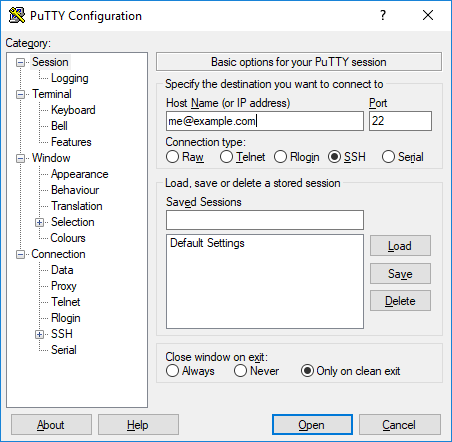
\includegraphics[width=0.7\textwidth]{chapters/12-auth/img/putty.png}
  \caption{PuTTY}
  \label{fig:sec:putty}
\end{figure}

\begin{figure}[!htbp]
  \centering
  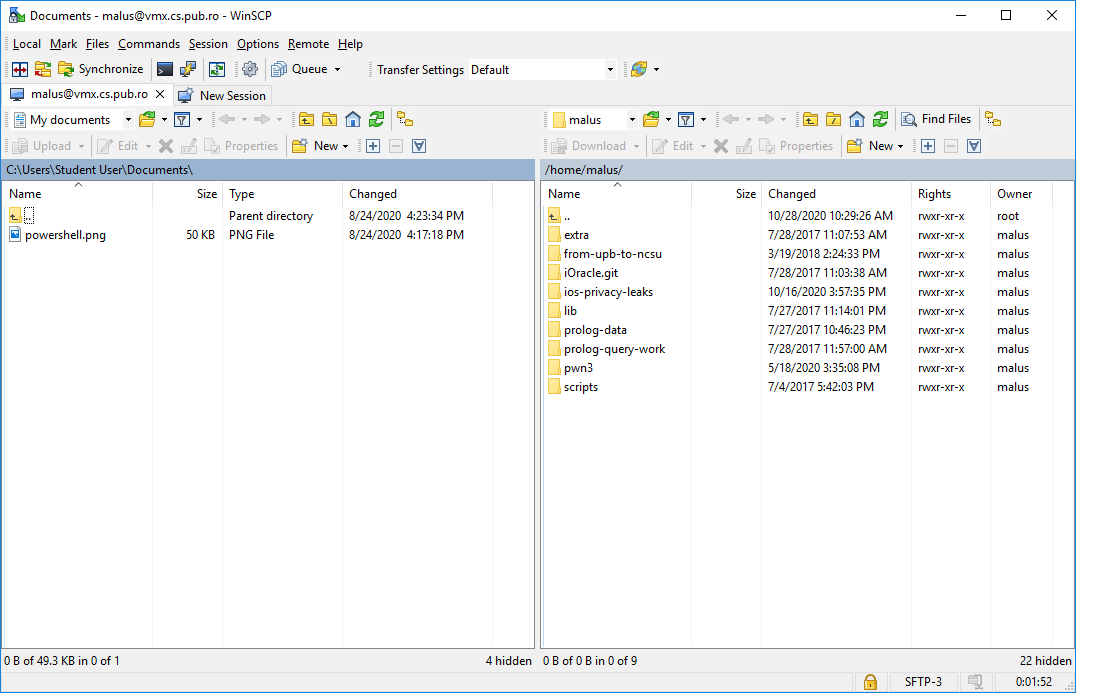
\includegraphics[width=0.7\textwidth]{chapters/12-auth/img/winscp.png}
  \caption{WinSCP}
  \label{fig:sec:winscp}
\end{figure} 